
\hkapitola{Datové typy, výrazy, základní konstrukce}

\begin{frame}[fragile]
%\footnotesize
\begin{tabular}{ccc}
\textbf{Java} & \textbf{C/C++} & \textbf{C\#} \\
\hline
\multicolumn{3}{c}{\textbf{Výstup}} \\
bytecode & nativní kód & MSIL (bytecode) \\
\hline
\multicolumn{3}{c}{\textbf{Správa paměti}} \\
garbage collector & ručně & garbage collector \\
reference & ukazatele, reference & ukazatele, reference \\
\hline
\multicolumn{3}{c}{\textbf{Objektový model}} \\
jednoduchá dědičnost & vícenásobná dědičnost & jednoduchá dědičnost \\
& & vlastnosti, indexery, \\
& & delegáty, události \\
\hline
\multicolumn{3}{c}{\textbf{Přetěžování operátorů}} \\
\no & \yes & \yes \\
\hline
\multicolumn{3}{c}{\textbf{Organizace modulů}} \\
package & namespace & assembly,namespace \\
Maven, Gradle & \ldots & NuGet \\

\hline
\multicolumn{3}{c}{\textbf{Generické programování}} \\
genericita (type erasure) & šablony & genericita (reification) \\

\hline
\multicolumn{3}{c}{\textbf{Knihovna jazyka}} \\
java.lang, java.util, \ldots & C/C++, STL & java like \\
\end{tabular}
\end{frame}

\begin{frame}[fragile]
\begin{center}
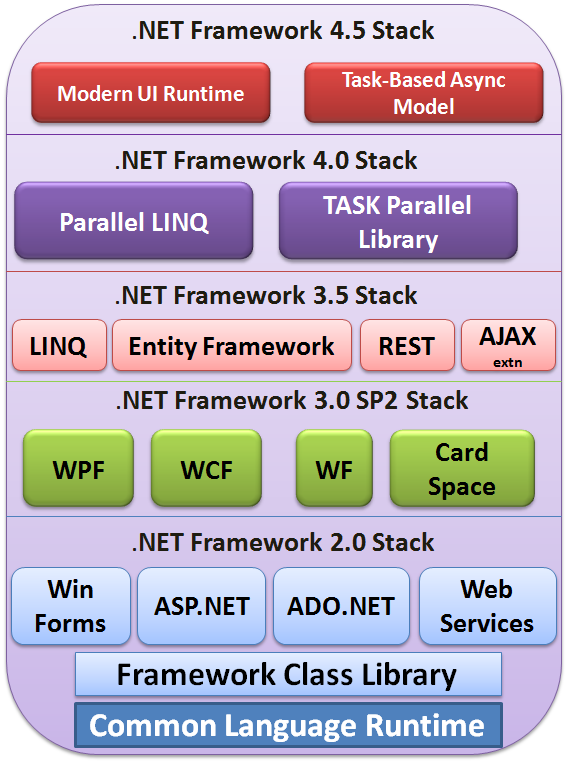
\includegraphics[height=\textheight]{img/dotnet_framework_stack.png}
\end{center}
\end{frame}

\begin{frame}[fragile]
\begin{center}
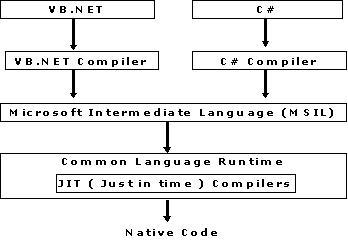
\includegraphics[width=\textwidth]{img/msil_code.jpg}
\end{center}
\end{frame}


\begin{frame}[fragile]
\begin{center}
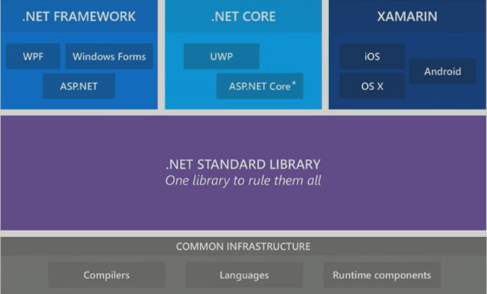
\includegraphics[width=\textwidth]{img/net_standard.png}
\end{center}
\end{frame}

\begin{frame}[fragile]
\begin{bitemize}{C\#}
\item kompilovaný jazyk (MSIL - mezikód)
\begin{itemize}
\item do nativního kódu je převeden runtime pomocí JIT
\end{itemize}
\item statické (i dynamické) typování
\item správa dynamické paměti pomocí garbage collectoru
\item základní knihovna podobná Javovské
\item inspirován Javou, C/C++, \ldots
\item aktuální verze C\# 7.2
\item standard a některé komponenty uvolněny pod open source licencemi
\item podpora pro non-Windows platformy pomocí Mono, nově .NET Core

\end{bitemize}
\end{frame}


\begin{frame}[fragile]
\begin{exampleblock}{Hello world!}
\begin{lstlisting}[basicstyle=\small]
using System;
using System.Collections.Generic;
using System.Linq;
using System.Text;
using System.Threading.Tasks;

namespace ConsoleApplication1
{
    class Program
    {
        static void Main(string[] args)
        {
            Console.WriteLine("Hello World!");
        }
    }
}
\end{lstlisting}
\end{exampleblock}
\end{frame}


\begin{frame}[fragile]
\begin{exampleblock}{Hello world! a dokumentační komentáře}
\begin{lstlisting}[basicstyle=\small]
namespace ConsoleApplication1
{
    /// <summary>
    /// Hlavni program.
    /// </summary>
    class Program
    {
        /// <summary>
        /// Main metoda
        /// </summary>
        /// <param name="args">argumenty prikazove radky</param>
        static void Main(string[] args)
        {
            Console.WriteLine("Hello World!");
        }
    }
}
\end{lstlisting}
\end{exampleblock}
\end{frame}

%\pkapitola{Coding conventions}

\begin{frame}[fragile]
\vfill
\begin{bitemize}{Coding conventions}
\item C\# definuje řadu doporučení a pravidel, jakým stylem by měl být psán a formátován kód
\item Základní doporučení:
\begin{itemize}
\item \color{green!50!black}VeřejnéTypy, Třídy, Struktury, Metody, Vlastnosti, \ldots začínají velkým písmenem, používá se PascalCase
\item \color{blue}privátníAtributy, parametryMetod, lokálníProměnné, \ldots začínají malým písmenem, používá se camelCase
\item \color{red}nepoužívá se hungarian notation, prefix \lstinline|m_|, \ldots
\end{itemize}

\end{bitemize}
\vfill
\begin{yesblock}
\begin{lstlisting}
class CarFactory { }
struct StudentRecord { }

public void GetElementAt(int elementIndex) { }

private string name;
\end{lstlisting}
\end{yesblock}
\vfill
\end{frame}



\kapitola{Proměnné, datové typy}


\begin{frame}[fragile]
\vfill
\begin{block}{Primitivní datové typy, proměnné}
\begin{itemize}
\item existují hodnotové a referenční datové typy
\item lze používat reference (na hodnotové typy, \lstinline|ref|)
\item lze používat ukazatele (\lstinline|unsafe|)
\item lokální proměnné se pojmenovávají dle camelCase (pocetZivotu, maximalniVykonMotoru)
\end{itemize}
\end{block}
\vfill
\begin{noteblock}{}
\begin{lstlisting}
nazevDatovehoTypu nazevPromenne [= inicializacniHodnota];
\end{lstlisting}
\end{noteblock}
\vfill
\end{frame}




\begin{frame}[fragile]
\begin{exampleblock}{Primitivní datové typy}
\begin{lstlisting}
// celá čísla
int x = 123;
// znakový typ
char c = 'c';
// desetinné typy
double d = 3.141592;
float f = 3.141592f;
// řetězec (není primitivní typ)
string s = "hello world";
// logický typ
bool b = true;
// desitkový desetinný typ
decimal dec = 3.333M;
           
Console.WriteLine("{0} {1} {2} {3} {4} {5} {6} {7} {8}", x, c, d, f, dec, va, nullablex, s, b);
Console.WriteLine($"{x}, {c}, {d}, {f}, {s}, {b}, {dec}");
\end{lstlisting}
\end{exampleblock}
\end{frame}

%// var - odvozeno kompilatorem z hodnoty na prave strane
%var va = 12356;
%// nullovatelny typ (standardni int + hodnota null navic)
%int? nullablex = null;


\begin{frame}[fragile]
\vfill
\begin{exampleblock}{Primitivní datové typy}
\begin{lstlisting}
// uint je 32 bitový bezznaménkový typ
uint bezznamenkovyInteger;
\end{lstlisting}
\end{exampleblock}
\vfill
\begin{bonusblock}{~}
\begin{lstlisting}
System.SByte int8; // sbyte
System.Int16 int16; // short
System.Int32 int32; // int
System.Int64 int64; // long

System.Byte uint8; // byte
System.UInt16 uint16; // ushort
System.UInt32 uint32; // uint
System.UInt64 uint64; // ulong

System.Single fSingle; // float
System.Double fDouble; // double
System.Decimal fDecimal; // decimal
\end{lstlisting}
\end{bonusblock}
\vfill
\end{frame}


\begin{frame}[fragile]
\begin{block}{Synonyma}
\begin{itemize}
\item Pozor na synonyma, je možné používat obojí, ale preferována je použití klíčového slova před názvem typu\ldots
\item \lstinline|string == String|
\item \lstinline|object == Object|
\item \lstinline|int == System.Int32|
\item Tedy používejte \lstinline|string, object, int|
\end{itemize}
\end{block}
\end{frame}

\begin{frame}[fragile]
\vfill
\begin{block}{Nulovatelné datové typy}
\begin{itemize}
\item \lstinline|datovyTyp?|
\item slouží jako \uv{rozšiřující modifikátor} pro uložení hodnoty \lstinline|null| do libovolného typu
\item objekt pak má vlastnosti \lstinline|HasValue, Value| a metodu \lstinline|GetValueOrDefault|
\end{itemize}
\end{block}
\vfill
\begin{yesblock}
\begin{lstlisting}
// int může nabývat hodnot -2147483648 až 2147483647
// co když chceme říct, že hodnota není?
int? nulovatelnyInt = null;

nulovatelnyInt = 100;
nulovatelnyInt = null;

\end{lstlisting}
\end{yesblock}
\vfill
\end{frame}




\begin{frame}[fragile]
\vfill
\begin{block}{var -- automatické odvození datového typu}
\begin{itemize}
\item \lstinline|var| umožňuje nechat kompilátor odvodit datový typ
\item nejedná se o dynamický typ, \lstinline|var| nabývá pouze konkrétního datového typu
\item umožňuje použití anonymních (objektových) datových typů 
\end{itemize}
\end{block}
\vfill
\begin{yesblock}
\begin{lstlisting}
var varPromenna = 123;
// varPromenna je int
varPromenna++;
// nelze: varPromenna = "abcd";
\end{lstlisting}
\end{yesblock}
\vfill
\end{frame}


\begin{frame}[fragile]
\frametitle{Výčtové typy}
\vfill
\begin{yesblock}
\begin{lstlisting}
enum VyctovyTyp
{
    Prvni, // = 0
    Druhy, // = 1
    Treti // = 2
}

Console.WriteLine($"{VyctovyTyp.Prvni}");
\end{lstlisting}
\end{yesblock}
\vfill
\begin{yesblock}
\begin{lstlisting}
enum VyctovyTyp
{
    Prvni = 10,
    Druhy, // = 11
    Treti // = 12
}
\end{lstlisting}
\end{yesblock}
\vfill
\end{frame}


\begin{frame}[fragile]
\frametitle{Výčtové typy -- bitové masky}
\begin{bonusblock}{~}
\begin{lstlisting}
[Flags] // atribut System.FlagsAttribute
enum Permissions
{
    Read = 0x01,
    Write = 0x02,
    Execute = 0x04
}

static void Main(string[] args)
{
    Permissions p = Permissions.Read | Permissions.Write;
    if (p.HasFlag(Permissions.Read))
    {
        Console.WriteLine($"{p}");
    }
}
\end{lstlisting}
\end{bonusblock}
\end{frame}


\kapitola{Výrazy}


\begin{frame}[fragile]
\begin{exampleblock}{Proměnné a výrazy/operátory}
\begin{lstlisting}
int x = 123;

// přiřazení, složené výrazy
// =, +, -, *, /, %, +=, -=, *=, /=, %=
x = 456;
x += 99;
x = x - 99;
x = x * x;
// inkrementace/dekrementace
x++;
--x;
// ternární operátor
x = (x % 2 == 0) ? x : 0;

Console.WriteLine($"{x}");
\end{lstlisting}
\end{exampleblock}
\end{frame}


\begin{frame}[fragile]
\begin{exampleblock}{Proměnné a výrazy/operátory}
\begin{lstlisting}
int x = 123;
int y = 456;

// porovnání
// >, <, >=, <=, ==, !=
bool vysledekVetsi = x > y;
bool vysledekShoda = x == y;

// bitové operátory
// &, |, ^, >>, <<
int z = x & (y << 5);

\end{lstlisting}
\end{exampleblock}
\end{frame}



\begin{frame}[fragile]
\vfill
\begin{exampleblock}{Konverze datového typu -- kulaté závorky}
\begin{lstlisting}[basicstyle=\small]
double dbl = 123.45;
int ine = (int)dbl;
\end{lstlisting}
\end{exampleblock}
\vfill
\begin{exampleblock}{~}
\begin{lstlisting}[basicstyle=\small]
Parent parent = new Child();
Child child;

// vyvolá InvalidCastException pokud objekt nebude typu Child
child = (Child)parent; 
\end{lstlisting}
\end{exampleblock}
\vfill
\end{frame}





\begin{frame}[fragile]
\begin{exampleblock}{Konverze datového typu -- as, is}
\begin{lstlisting}[basicstyle=\small]
Parent parent = new Child();
Child child;

// null pokud nebude daného typu
child = parent as Child; 

// is - C# obdoba operátoru instanceof z Javy
if (parent is Child)
{
    Child cld = (Child)parent;
    cld.Action();
}

// C# 7 - umožňuje rovnou deklarovat proměnnou
if (parent is Child chd)
{
    chd.Action();
}
\end{lstlisting}
\end{exampleblock}
\end{frame}




\begin{frame}[fragile]
\begin{bonusblock}{Konverze datového typu -- reflexe + typeof}
\begin{lstlisting}[basicstyle=\small]
Parent parent = new Child();
Child child;

if (parent.GetType() == typeof(Child)) 
{
    child = (Child)parent;
}
\end{lstlisting}
\end{bonusblock}
\end{frame}



\begin{frame}[fragile]
\begin{exampleblock}{Null operátory}
\begin{lstlisting}
int? a = null;

// ??
int b = a ?? -1;
// a == null? potom b = -1
// a != null? potom b = a

// ?.
object o = null;
o?.ToString();
// o == null? potom nic nedělej
// o != null? potom zavolej ToString()

// ?[]
int[] array = null;
int? x = array?[0];
\end{lstlisting}
\end{exampleblock}
\vfill
\begin{yesblock}
\begin{lstlisting}
var value = firstObject?.secondObject?.maybeArray?[0] ?? "default";
\end{lstlisting}
\end{yesblock}
\end{frame}



\begin{frame}[fragile]
\begin{bonusblock}{Přetečení/podtečení -- checked blok}
\begin{lstlisting}
int i = 10, j = 0;
i = i / j; // vyvolá DivideByZeroException

(i, j) = (int.MaxValue, int.MinValue); // Tuples/n-tice C# 7
i++;
j--;
Console.WriteLine($"{i} {j}");
// i == -2147483648 == int.MinValue
// j == 2147483647 == int.MaxValue

(i, j) = (int.MaxValue, int.MinValue);
checked
{
    i++; // vyvolá OverflowException
    j--; // vyvolá OverflowException
}
\end{lstlisting}
\end{bonusblock}
\end{frame}


\pkapitola{Základní řídící konstrukce}



\begin{frame}[fragile]
\vfill
\begin{block}{Rozhodování}
\begin{itemize}
\item syntax stejná jako Java/C/C++
\item podmínka musí být vyhodnocena na typ \lstinline|bool|
\end{itemize}
\end{block}
\vfill
\begin{yesblock}
\begin{lstlisting}
int x = 123;
if (x > 10)
{
    Console.WriteLine("x > 10");
}
\end{lstlisting}
\end{yesblock}
\vfill
\begin{noblock}
\begin{lstlisting}
int x = 123;
if (x)
{
    Console.WriteLine("error");
}
\end{lstlisting}
\end{noblock}
\vfill
\end{frame}

\begin{frame}[fragile]
\begin{yesblock}
\begin{lstlisting}
int x = 123;
if (x > 10)
{
    Console.WriteLine("x > 10");
}
else
{
    Console.WriteLine("x <= 10");
}
\end{lstlisting}
\end{yesblock}
\end{frame}





\begin{frame}[fragile]
\vfill
\begin{block}{Cykly}
\begin{itemize}
\item \lstinline|while, do-while, for, foreach|
\item syntax shodná
\item \lstinline|foreach| lze využívat na pole a kolekce
\item podporováno řízení cyklů \lstinline|break, continue|
\end{itemize}
\end{block}
\vfill
\begin{yesblock}
\begin{lstlisting}
int x = 123;
for (int i = 0; i < x; i++) 
{
    Console.WriteLine("{0}", i);
}
\end{lstlisting}
\end{yesblock}
\vfill
\end{frame}



\begin{frame}[fragile]
\vfill
\begin{yesblock}
\begin{lstlisting}
do
{
    x--;
} while (x > 0);
\end{lstlisting}
\end{yesblock}
\vfill
\begin{yesblock}
\begin{lstlisting}
while (x < 10)
{
    x++;
}
\end{lstlisting}
\end{yesblock}
\vfill
\end{frame}




\begin{frame}[fragile]
\begin{yesblock}
\begin{lstlisting}
int x = 123;
while (true)
{
    if (x == 200)
        continue;

    if (x == 300)
        break;
    
    x++;
}
\end{lstlisting}
\end{yesblock}
\end{frame}





\begin{frame}[fragile]
\vfill
\begin{block}{Switch}
\begin{itemize}
\item syntax shodná
\item nelze propadávat z jednoho \lstinline|case| do druhého, je nutné explicitně skočit \lstinline|goto case 123|
\item nepovinná větev \lstinline|default| pro ostatních hodnot
\end{itemize}
\end{block}
\vfill
\begin{bonusblock}{~}
\begin{itemize}
\item od C\# 7 podpora pattern matching
\begin{itemize}
\item umožňuje rozlišit datový typ objektu (lze dále definovat podmínku)
\item \lstinline|case string s when s.Contains("foobar"):|
\item \lstinline|case int n when n > 100:|
\item \lstinline|case int n:|
\end{itemize}
\end{itemize}
\end{bonusblock}
\vfill
\end{frame}





\begin{frame}[fragile]
\begin{yesblock}
\begin{lstlisting}
int x = 123;
switch (x)
{
    case 0: 
        Console.WriteLine("0");
        break;

    case 1:
        Console.WriteLine("1");
        //goto case 0; // preskok na 0
        //goto default; // preskok na default
        break;

    default:
        Console.WriteLine("...");
        break;
}
\end{lstlisting}
\end{yesblock}
\end{frame}




\kapitola{Pole}

\begin{frame}[fragile]
\begin{block}{Pole}
\begin{itemize}
\item pole je objekt
\item C\# umožňuje vytvářet 3 typy polí
\begin{itemize}
\item jednorozměrná pole
\item vícerozměrná pole (pravidelná)
\item vícerozměrná pole (nepravidelná, jagged array)
\end{itemize}

\item syntax obdobný Javě, hranaté závorky, indexování prvků od nuly, přístup mimo rozsah pole vyvolá výjimku
\end{itemize}
\end{block}
\end{frame}

\begin{frame}[fragile]
\frametitle{Jednorozměrné pole}
\begin{yesblock}
\begin{lstlisting}
int[] pole;
pole = new int[10];

pole[0] = 10;
pole[1] = 20;
//pole[10] = 15; // IndexOutOfRangeExpection

int pocetPrvkuPole = pole.Length;

Console.WriteLine($"{pocetPrvkuPole} {pole.Length} {pole[0]}{pole[1]}");
\end{lstlisting}
\end{yesblock}
\end{frame}



\begin{frame}[fragile]
\frametitle{Vícerozměrné pole (pravidelné)}
\begin{yesblock}
\begin{lstlisting}
int[,] pole = new int[2,3];

pole[0, 0] = 1;
pole[0, 1] = 2;
pole[0, 2] = 3;
pole[1, 0] = 4;
pole[1, 1] = 5;
pole[1, 2] = 6;

int pocetPrvkuVPoli = pole.Length; // == 2*3 == 6
int pocetPrvkuVPrvniDimenzi = pole.GetLength(0); // == 2
int pocetPrvkuVDruheDimenzi = pole.GetLength(1); // == 3

Console.WriteLine($"{pocetPrvkuVPoli} {pole.Length} {pocetPrvkuVPrvniDimenzi} {pocetPrvkuVDruheDimenzi} {pole[0, 0]} {pole[0, 1]}");
\end{lstlisting}
\end{yesblock}
\end{frame}


\begin{frame}[fragile]
\frametitle{Vícerozměrné pole (pravidelné)}
\begin{yesblock}
\begin{lstlisting}
int[] pole1D = new int[2];
int[,] pole2D = new int[2,3];
int[,,] pole3D = new int[2,3,5];
int[,,,] pole4D = new int[2,3,5,6];
int[,,,,] pole5D = new int[2,3,5,6,7];
\end{lstlisting}
\end{yesblock}
\end{frame}



\begin{frame}[fragile]
\frametitle{Vícerozměrné pole (nepravidelné, jagged array)}
\begin{yesblock}
\begin{lstlisting}
int[][] jaggedArray = new int[3][];
jaggedArray[0] = new int[2];
jaggedArray[1] = new int[3];
jaggedArray[2] = new int[4];

jaggedArray[0][0] = 1;
jaggedArray[0][1] = 2;
jaggedArray[1][0] = 3;
jaggedArray[1][1] = 4;
jaggedArray[1][2] = 5;

Console.WriteLine($"{jaggedArray[0][0]} {jaggedArray[0][1]}");
\end{lstlisting}
\end{yesblock}
\end{frame}





\kapitola{Základní konzolové příkazy}


\begin{frame}[fragile]
\vfill
\begin{block}{Výstupní parametry metod}
Umožňují předat volající funkci další výsledky.
\end{block}
\vfill
\begin{yesblock}
\begin{lstlisting}
static void OutMethod(int a, out int b, out int c)
{
    b = 2 * a;
    c = 3 * a;
}

static void Main(string[] args)
{
    int a = 123;
    int b, c;
    OutMethod(a, out b, out c);
    Console.WriteLine("{0} {1} {2}", a, b, c);
}
\end{lstlisting}
\end{yesblock}
\vfill
\end{frame}


\begin{frame}[fragile]
\vfill
\begin{block}{Referenční parametry metod}
Parametry funkce předávané "odkazem".
\end{block}
\vfill
\begin{yesblock}
\begin{lstlisting}
static void RefMethod(int a, ref int b)
{
    b = b * a;
}

static void Main(string[] args)
{
    int a = 123;
    int b = 456;
    RefMethod(a, ref b);
    Console.WriteLine("{0} {1}", a, b);
}
\end{lstlisting}
\end{yesblock}
\vfill
\end{frame}



\begin{frame}[fragile]
\vfill
\begin{exampleblock}{Konverze string $\rightarrow$ int/double/\ldots}
\begin{lstlisting}
string str = "123";
// Parse - vyvolá FormatException, pokud parametr neobsahuje řetězec s číslem
int istr = int.Parse(str);
\end{lstlisting}
\end{exampleblock}
\vfill
\begin{exampleblock}{Konverze string $\rightarrow$ int/double/\ldots}
\begin{lstlisting}
// TryParse - vrací bool (úspěch/neúspěch konverze), zkonvertovaná hodnota je vrácena výstupním parametrem
int istr2;
bool uspech = int.TryParse(str, out istr2);
if (uspech) 
{
    Console.WriteLine(istr2);
}
\end{lstlisting}
\end{exampleblock}
\vfill
\end{frame}


\begin{frame}[fragile]
\vfill
\begin{exampleblock}{Také lze využít třídu System.Convert}
\begin{lstlisting}
int valueInt = Convert.ToInt32("123456");
double valueDouble = Convert.ToDouble("3,1415");
\end{lstlisting}
\end{exampleblock}
\vfill
\begin{exampleblock}{Konverze int/double/\ldots $\rightarrow$ string}
\begin{lstlisting}
int i = 123;

string s = i.ToString();
// lze také:
// string s = 123.ToString();
\end{lstlisting}
\end{exampleblock}
\vfill
\end{frame}


\begin{frame}[fragile]
\begin{exampleblock}{Třída System.Console}
\begin{lstlisting}
Console.Write(...); // vytiskne text
Console.WriteLine(...); // vytiskne text a odradkuje
Console.Read(); // nacte znak
Console.ReadKey(); // nacte stisk klavesy
Console.ReadLine(); // nacte radek textu
\end{lstlisting}
\end{exampleblock}
\end{frame}
